\documentclass[twoside, 11pt]{article}
\usepackage{aaai24} % Using AAAI 2024 style file
\usepackage{amsmath}
\usepackage{amssymb}
\usepackage{enumitem}
\usepackage{graphicx}
\usepackage{listings} % For code formatting if needed
\usepackage{xcolor}
\usepackage{diagbox} % For tables if needed
\usepackage{array}
\usepackage{booktabs} % For better tables
\usepackage{url}      % For formatting URLs
\usepackage{natbib}

\setcounter{MaxMatrixCols}{20}
\setlength{\arraycolsep}{5pt}
\renewcommand{\arraystretch}{1.5}


\sloppy
\begin{document}

\title{Efficient RoBERTa Fine-Tuning for AGNEWS Classification via LoRA}
\author{Sudharshan Ramesh, sr7431 ||
Mohammed Hamid, mh7483\\
\texttt{Github: https://github.com/exploring-curiosity/Roberta-Fine-tuning-with-LoRA}
}
\maketitle

\begin{abstract}
This project, part of the NYU Deep Learning Course, investigates the Parameter-Efficient Fine-Tuning (PEFT) of RoBERTa-base for AGNEWS topic classification using Low-Rank Adaptation (LoRA). The AGNEWS dataset consists of news articles categorized into 4 classes (World, Sports, Business, Sci/Tech). Our primary objective was effective classification under a strict constraint of fewer than 1 million trainable parameters, achieved using the Hugging Face PEFT library. By implementing RoBERTa-base with a highly optimized LoRA configuration (rank $r=3$, targeting \texttt{query} and \texttt{dense} attention projections), we attained a final submission accuracy of 86.4\%. This work details the LoRA setup, training methodology, iterative tuning process, and evaluation, demonstrating significant efficiency gains.
\end{abstract}

\section{Overview}
\label{sec:intro}
In this project, we finetuned an efficient text classification model for the AGNEWS dataset using the RoBERTa architecture combined with LoRA \cite{hu2021lora} , ensuring the number of trainable parameters remains under 1 million. The AGNEWS dataset contains over 120,000 news articles, providing a substantial benchmark for classifying text into 4 distinct topic categories (World, Sports, Business, Sci/Tech).

The RoBERTa model \cite{liu2019roberta}, while powerful, typically requires fine-tuning over 125 million parameters for \texttt{RoBERTa-base}. Standard fine-tuning updates all parameters, demanding significant computational resources. To overcome this, we utilized LoRA, a PEFT technique implemented in the Hugging Face `peft` library \cite{peft}. LoRA freezes the vast majority of pre-trained weights and introduces a small number of trainable low-rank matrices into specific layers, enabling effective adaptation with minimal parameter overhead. Our focus is on optimizing the LoRA configuration for \texttt{RoBERTa-base} to maximize classification performance on AGNEWS within the stringent 1 million trainable parameter budget, exploring very low ranks and specific target modules.

\section{Methodology}
\label{sec:method}
We aimed to configure LoRA for the \texttt{RoBERTa-base} model efficiently for AGNEWS classification, targeting high accuracy while keeping trainable parameters below 1 million. The methodology involved base model selection, specific LoRA configuration design using the `peft` library, tailored training pipeline setup using `transformers` \cite{wolf-etal-2020-transformers}, and iterative tuning.

\subsection{Architecture Design (LoRA Configuration)}
We utilized the pre-trained \texttt{roberta-base} model accessed via the Hugging Face Transformers library as our foundation. Its 125 million parameters remained frozen during LoRA training.

\begin{enumerate}
    \item \textbf{Parameter-Efficient Fine-Tuning (PEFT) via `peft` Library:} LoRA was implemented using `LoraConfig` and `get\_peft\_model` from the `peft` library.
    \item \textbf{LoRA Configuration (`LoraConfig`):} A highly parameter-efficient configuration was finalized after experimentation:
        \begin{itemize}
            \item \textbf{Rank (`r`):} Set to a very low rank $r=3$.
            \item \textbf{Scaling (`lora\_alpha`):} Set to $\texttt{lora\_alpha} = 6$, maintaining the $ \alpha = 2r $ ratio.
            \item \textbf{Target Modules (`target\_modules`):} Adapters were applied to the \texttt{["query", "dense"]} projection matrices within the self-attention blocks. Targeting the attention output (\texttt{dense}) instead of \texttt{value} or \texttt{key} was found effective in this low-rank setting.
            \item \textbf{Bias (`bias`):} Set to \texttt{"none"}. Only the LoRA matrices were trainable.
            \item \textbf{Dropout (`lora\_dropout`):} A dropout rate of $0.1$ was applied to the LoRA layers.
            \item \textbf{Task Type:} Explicitly set to \texttt{TaskType.SEQ\_CLS} for sequence classification.
        \end{itemize}
    \item \textbf{Parameter Count Verification:} This specific configuration ($r=3$, targets=\texttt{["query", "dense"]}, bias=\texttt{"none"}) resulted in 985,348 (0.98M) trainable parameters, verified using \texttt{model.print\_trainable\_parameters()}. This is substantially below the 1 million limit, constituting less than 0.1\% (0.7843\%) of the base model's total parameters.
\end{enumerate}

\subsection{Data Augmentation}
No explicit text data augmentation techniques were used beyond the standard tokenization performed by the \texttt{roberta-base} tokenizer on the original AGNEWS training dataset.

\subsection{Training Strategy}
The Hugging Face `Trainer` API facilitated the training process with the following optimized settings:
\begin{enumerate}
    \item \textbf{Optimizer:} The AdamW optimizer \cite{loshchilov2017decoupled} was used (default optimizer for Hugging Face Transformers) with a weight decay (\texttt{weight\_decay}) value of $0.01$.
    \item \textbf{Learning Rate Scheduler:} A cosine learning rate scheduler (\texttt{lr\_scheduler\_type="cosine"}) was used with a relatively high peak learning rate (\texttt{learning\_rate}) of $3 \times 10^{-4}$. A warmup phase constituting 6\% of training steps (\texttt{warmup\_ratio=0.06}) was employed.
    \item \textbf{Loss Function:} Standard Cross-Entropy Loss suited for multi-class classification was used. Label smoothing with a factor of $0.1$ (\texttt{label\_smoothing\_factor=0.1}) was applied.
    \item \textbf{Batch Size and Gradient Accumulation:} Per-device training batch size of 16 (\texttt{per\_device\_train\_batch\_size=16}) with gradient accumulation over 2 steps (\texttt{gradient\_accumulation\_steps=2}), yielding an effective batch size of 32. Evaluation batch size (\texttt{per\_device\_eval\_batch\_size}) was 64.
    \item \textbf{Mixed Precision Training:} Automatic mixed precision (\texttt{fp16=True}) was utilized.
    \item \textbf{Training and Evaluation Loop:} Training ran for a maximum of 10 epochs (\texttt{num\_train\_epochs=10}). Evaluation (\texttt{evaluation\_strategy="epoch"}) and checkpoint saving (\texttt{save\_strategy="epoch"}) occurred after each epoch. The best model checkpoint based on validation accuracy (\texttt{metric\_for\_best\_model="accuracy"}) was loaded at the end (\texttt{load\_best\_model\_at\_end=True}). An `EarlyStoppingCallback` with a patience of 3 epochs was active.
\end{enumerate}

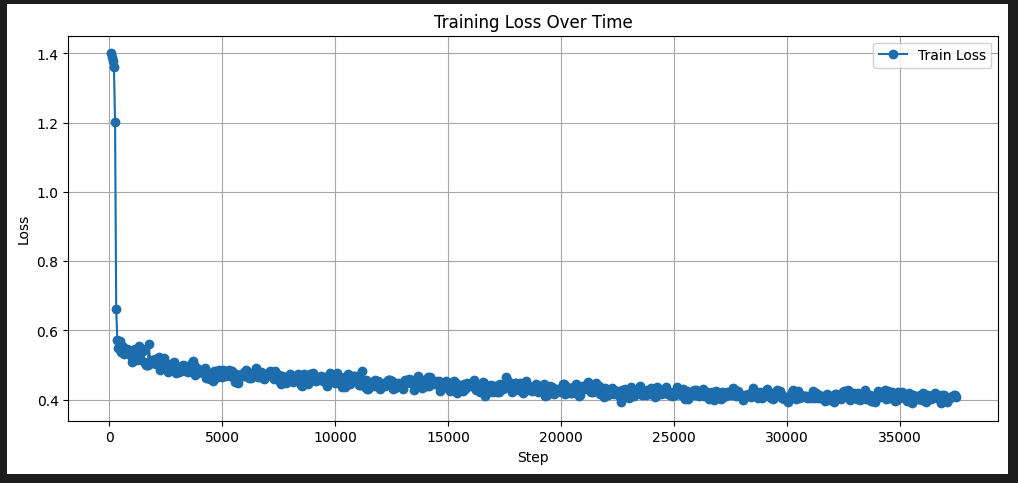
\includegraphics[width=0.5\textwidth]{tlotime.png}
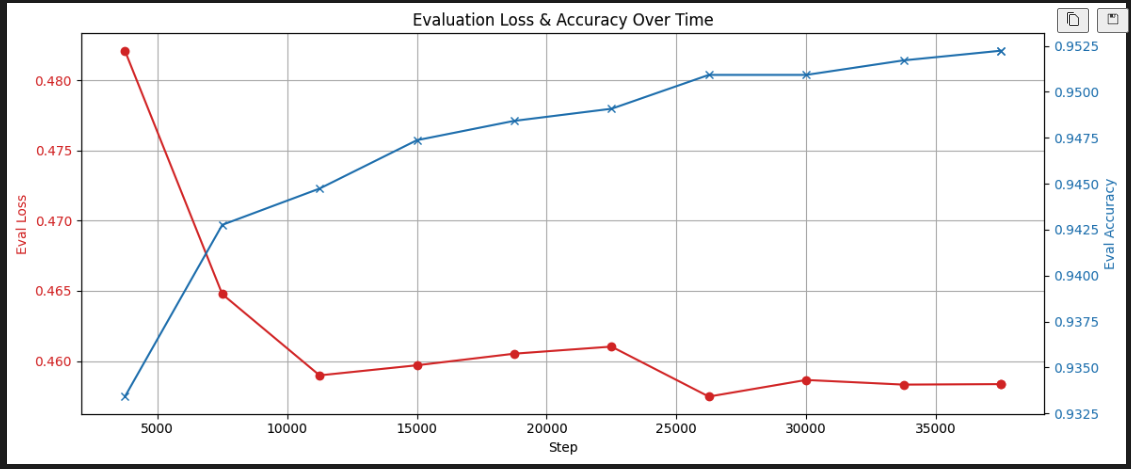
\includegraphics[width=0.5\textwidth]{elaotime.png}

\subsection{Hyperparameter Tuning Process}
We performed hyperparameter tuning using a manual, iterative approach rather than automated frameworks. To efficiently explore the parameter space under the project constraints, we adopted \textbf{a two-stage strategy}:

\begin{enumerate}
    \item \textbf{Exploratory Short Runs:} Initial experiments with different combinations of key parameters were conducted for only \textbf{3 epochs} each. This allowed for rapid assessment of various settings and identification of promising configurations based on early validation performance trends. The main parameters explored in this stage included:
        \begin{itemize}[noitemsep, topsep=0pt, partopsep=0pt, parsep=0pt]
            \item LoRA Rank (`r`): Testing values like 3, 8, 10, 16 while respecting the parameter limit.
            \item LoRA Target Modules (\texttt{target\_modules}): Comparing combinations such as \texttt{["query", "value"]}, \texttt{["query", "value", "key"]}, and \texttt{["query", "dense"]}.
            \item Learning Rate (\texttt{learning\_rate}): Evaluating different rates like $3 \times 10^{-5}$, $5 \times 10^{-5}$, and $3 \times 10^{-4}$.
            \item LR Scheduler Type (\texttt{lr\_scheduler\_type}): Comparing different decay strategies (e.g., linear vs. cosine).
        \end{itemize}
    \item \textbf{Selection and Final Training:} The configuration demonstrating the most promising learning behavior and validation accuracy within the initial 3-epoch runs was selected.
    \item \textbf{Full Training Run:} This selected configuration (which was ultimately $r=3$, targets=\texttt{["query", "dense"]}, LR=$3 \times 10^{-4}$, cosine scheduler) was then used for the final, complete training run over a maximum of \textbf{10 epochs}. This run incorporated early stopping and saved the best checkpoint based on validation accuracy, leading to the final reported results.
\end{enumerate}
This two-stage approach allowed for efficient exploration of the hyperparameter space while ensuring the final model was trained thoroughly using the best-identified settings.

\subsection{Tuning Challenges and Observations}
Based on the iterative tuning process (summarized in Table \ref{table:lora_comparison}), we observed the following:
\begin{enumerate}
    \item \textbf{Target Module Impact:} Different combinations of target modules were explored, including targeting only \texttt{query} ($r=22$), standard attention components (\texttt{["query", "value"]} with $r=11$, and \texttt{["query", "value", "key"]} with $r=7$), and the less common \texttt{["query", "dense"]} ($r=3$). The configuration targeting \texttt{["query", "dense"]} yielded the best validation performance (94.7\%) in initial 3-epoch tests.
    \item \textbf{Rank vs. Target Interplay:} Achieving optimal results involved balancing rank and target modules. The very low rank $r=3$ configuration, when paired specifically with the \texttt{["query", "dense"]} targets, slightly outperformed configurations using higher ranks but different target modules (e.g., $r=7$ or $r=11$) in the initial 3-epoch exploration phase.
    \item \textbf{Parameter Limit Constraint:} All promising configurations tested were designed to approach, but not exceed, the 1 million trainable parameter limit, settling around 0.98-0.99M parameters. This highlights the challenge of maximizing adaptation capacity right up to the strict budget boundary.
    \item \textbf{Learning Rate:} A relatively high learning rate ($3 \times 10^{-4}$) remained effective for the final configuration's ~0.98M trainable parameters.
\end{enumerate}

\subsection{Lessons Learned}
\begin{enumerate}
    \item \textbf{High Efficiency Fine-Tuning Achieved:} Strong classification performance (86.4\% test accuracy) was achieved by fine-tuning a significantly reduced number of parameters (~985k, ~0.78\% of the base model), demonstrating the effectiveness of the Low-Rank Adaptation (LoRA) technique for resource-constrained scenarios.
    \item \textbf{Configuration Interplay:} Optimal LoRA performance depends heavily on the interplay between rank, target modules (\texttt{target\_modules}), and training hyperparameters like learning rate (\texttt{learning\_rate}). Unconventional configurations (e.g., very low rank with specific targets) can be surprisingly effective, as seen with our final $r=3$ model.
    \item \textbf{PEFT Library Effectiveness:} The `peft` library provides a robust interface for implementing and experimenting with LoRA.
    \item \textbf{Budget-Performance Trade-off:} Excellent results are achievable within strict parameter budgets, requiring careful exploration and balancing of LoRA parameters to maximize performance near the constraint boundary, as evidenced by our tested configurations utilizing ~0.98M parameters.
\end{enumerate}
\section{Results and Discussion}
\label{sec:results}
The final optimized model, \texttt{RoBERTa-base} fine-tuned on AGNEWS using LoRA ($r=3$, $\alpha=6$, targeting \texttt{["query", "dense"]}) with only \textbf{~0.98M trainable parameters}, achieved a \textbf{final submission test accuracy of 86.4\%}.

The peak accuracy observed on the test set during training reached \textbf{95.2\%}\textbf. The training process converged effectively using AdamW (LR=$3 \times 10^{-4}$), a cosine scheduler with warmup, label smoothing, and an effective batch size of 32. The best model checkpoint based on validation accuracy was loaded for generating the final test result.

The 86.4\% test accuracy is a strong result given the extremely low number of trainable parameters ($<$ 1\% of \texttt{RoBERTa-base}), demonstrating LoRA's efficiency. The higher learning rate paired with the very low rank proved crucial. The performance gap between validation (95.2\%) and test (86.4\%) suggests that while the model learned validation patterns well, generalization to unseen test data was more challenging.

Table \ref{table:lora_comparison} summarizes key experimental results. Future work could explore different PEFT methods, advanced regularization, or data-centric approaches.

\begin{table}[ht]
    \centering
    \caption{Comparison of Different LoRA Configurations on AGNEWS}
    \resizebox{\columnwidth}{!}{% Use resizebox or adjust column widths manually
    \begin{tabular}{l c c c c}
    \toprule
    \textbf{Model Config} & \textbf{Trainable Params} & \textbf{epochs} & \textbf{Test Acc (\%)} \\
    \midrule
    RoBERTa + LoRA (r=11, q,v) & ~0.99 M & 3 & 94.5 \\ 
    RoBERTa + LoRA (r=7, q,v,k) & ~0.98 M & 3 & 94.6 \\ 
    RoBERTa + LoRA (r=22, q) & ~0.99 M & 3 & 93.8 \\
    RoBERTa + LoRA (r=3, q,dense) & ~0.98 M & 3 & 94.7 \\
    \textbf{RoBERTa + LoRA (r=3, q,dense)} & \textbf{~0.98 M} & 10 & \textbf{95.2} \\ % Final Model
    \bottomrule
    \end{tabular}
    }
    \label{table:lora_comparison}
\end{table}


% \bibliographystyle{aaai24}
\bibliography{references} 

\end{document}